\documentclass[parskip=full]{scrartcl}

\usepackage[utf8]{inputenc}			% Umlaute, Sonderzeichen
\usepackage[ngerman]{babel}			% deutsche Sprache
\usepackage{enumitem}				% Listen
\usepackage{graphicx}				% Grafiken
\usepackage{hyperref}				% Hyperlinks
\usepackage[nonumberlist]{glossaries}		% Glossar
\usepackage{amsmath}
\usepackage{pdfpages}				% PDF einbinden


% Hurenkinder und Schusterjungen verhindern
\clubpenalty10000
\widowpenalty10000
\displaywidowpenalty=10000

\DeclareRobustCommand{\glossfirstformat}[1]{\textit{#1}}	% der erste Verweis im Dokument auf ...
\renewcommand*{\glsdisplayfirst}[4]{\glossfirstformat{#1#4}}	% ... einen Glossarbegriff wird kursiv markiert

% Kriterien sollen nicht kursiv erscheinen
\makeatletter
\renewcommand{\@begintheorem}[2]{\trivlist
	\item[\hskip \labelsep{\bfseries #1\ #2}]}
\makeatother


\makenoidxglossaries

\newglossaryentry{RasPi}{
	name=Raspberry Pi,
	plural=Raspberry Pis,
	description={Der Raspberry Pi ist ein Einplatinencomputer. In diesem Projekt dient der Raspberry Pi als Hardwareplattform, um Messwerte aus angeschlossenen Sensoren auszulesen}
}

\newglossaryentry{PhyPiDAQ}{
	name=PhyPiDAQ,
	description={PhyPiDAQ ist ein Framework zur Erfassung und Analyse von Messwerten mit einem Raspberry Pi. Siehe auch Abschnitt 4.3 ,,PhyPiDAQ`` sowie \url{https://github.com/GuenterQuast/PhyPiDAQ}}
}

\newglossaryentry{Science Labs}{
	name=Science Labs,
	description={Ein Science Lab ist ein Arbeitsplatz, welcher Schülern ermöglicht, wissenschaftliche Forschungen unter kontrollierten Bedingungen durchzuführen} 
}

\newglossaryentry{opensource}{
	name=Open Source,
	description={Software, deren Quelltext öffentlich eingesehen eingesehen werden kann, wird als ,,Open Source`` bzw. ,,quelloffen`` bezeichnet} 
}

\newglossaryentry{osl2}{
	name=OSL\textsuperscript{2},
	description={Open-Source-Lehrsoftware-Labor, siehe \url{https://formal.iti.kit.edu/projects/oslsl/?lang=de}}
}

\newglossaryentry{dragdrop}{
	name=Drag and Drop,
	description={Methode, um mit grafischen Benutzeroberflächen zu interagieren. Dabei wird ein Objekt erst mit der Maus festgehalten und an einen anderen Ort gezogen. Durch das Lösen der Maustaste wird das Objekt platziert}
}

\newglossaryentry{click}{
	name=Click,
	description={Betätigen der linken Maustaste}
}

\newglossaryentry{transformation}{
	name=Transformation,
	plural={Transformationen},
	description={Bausteine vom Typ Transformation haben einen oder mehrere Eingänge sowie einen oder mehrere Ausgänge. Für jeden Ausgang kann  ein Transformationsbaustein eine Vorschrift zur Berechnung eines Ausgangswertes aus einem Satz von Eingangswerten beinhalten. Eine Berechnungsvorschrift soll durch eine mathematische bzw. logische Funktionen oder durch eine programmtechnisch definierte Verarbeitung definiert werden können}
}

\newglossaryentry{konfigdata}{
	name=Konfigurationsdatei,
	plural=Konfigurationsdateien,
	description={Können das Messverhalten anpassen, beispielsweise die Anzahl der Messungen pro Zeiteinheit. Für jeden Sensor gibt es eine eigene Konfigurationsdatei}
}

\newglossaryentry{sensor}{
	name=Sensor,
	plural={Sensoren},
	description={Der Begriff ,,Sensor`` bezeichnet ein technisches Bauteil, welches physikalische Größen misst und analoge oder digitale Messwerte liefert. In unserer Anwendung werden Sensoren abstrakt als grafische Bausteine eines Messkonfiguration präsentiert. Ein solcher (logischer) Sensorbaustein muss alle Informationen referenzieren können, die zum Ansprechen eines tatsächlichen Sensors benötigt werden. Da ein Messgerät Ausgänge bzw. Messkanäle haben kann, muss ein Sensorbaustein mindestens einen oder auch mehrere Ausgänge haben. Eingänge besitzt ein Sensorbaustein nicht}
}

\newglossaryentry{messdaten}{
	name=Messdaten,
	description={Daten, welche die Anwendung von einem Sensor (über PhyPiDAQ-Schnittstelle) oder direkt aus einer Datei erhält}
}

\newglossaryentry{darstellung}{
	name=Darstellung,
	plural={Darstellungen},
	description={Bausteine vom Typ Darstellung haben einen oder mehrere Eingänge. Ein Darstellungsbaustein soll definieren können, wie ein Satz von Eingangswerten die Erstellung bzw. Aktualisierung einer Darstellung beeinflusst. Ausgänge besitzt ein Darstellungsbaustein nicht}
}

\newglossaryentry{python3}{
	name=Python 3,
	description={Python ist eine Skriptsprache, die auf dem Raspberry Pi als Standardsprache zur Programmierung vorgesehen ist. Python wurde zur Implementierung von PhyPiDAQ verwendet}
}

\newglossaryentry{JVM}{
	name={Java Virtual Machine},
	description={Die Java Virtual Machine (JVM) ist eine Plattform für die Ausführung von Java-Software, die von der Firma Oracle für alle gängigen Betriebssysteme bereitgestellt wird}
}

\newglossaryentry{DSGVO}{
	name=DSGVO,
	first={Datenschutz-Grundverordnung (DSGVO)},
	description ={Datenschutz-Grundverordnung der Europäischen Union vom 25. Mai 2018}
}

\newglossaryentry{Musskriterien}{
	name=Musskriterien,
	description ={Werden zusammen mit Soll- und Wunschkriterien bei der Abnahme eines Softwareprodukts überprüft und haben während der Entwicklung höchste Priorität. 
	Dass ein Musskriterium in den nachfolgenden Projektphasen nicht umgesetzt wird, ist nur dann zulässig, falls unerwartet unausweichliche Probleme bei der Umsetzung auftreten. 
	In diesem Fall ist es erforderlich, dass diese Probleme sehr genau dokumentiert werden}
}

\newglossaryentry{Sollkriterien}{
	name=Sollkriterien,
	description ={Werden zusammen mit Muss- und Wunschkriterien bei der Abnahme eines Softwareprodukts überprüft und haben während der Entwicklung mittlere Priorität. 
	Falls ein Sollkriterium umgesetzt werden kann, dann muss es nach Möglichkeit auch realisiert werden. 
	Falls ein Sollkriterium in den nachfolgenden Projektphasen nicht umgesetzt werden kann, so muss dies dokumentiert und begründet werden}
}

\newglossaryentry{Wunschkriterien}{
	name=Wunschkriterien,
	description ={Werden zusammen mit Muss- und Sollkriterien bei der Abnahme eines Softwareprodukts überprüft und haben während der Entwicklung eine niedrige Priorität. 
	Je nach Resourcenlage können sie nach Bearbeitung aller Muss- und Kannkriterien umgesetzt werden. 
	Falls ein Wunschkriterium nicht umgesetzt wird, so muss dies nicht begründet werden}
}

\newglossaryentry{Abgrenzungskriterien}{
	name=Abgrenzungskriterien,
	description ={Abgrenzungskriterien beschreiben Aspekte, die explizit nicht umgesetzt werden sollen}
}

\newglossaryentry{BenOber}{
	name=Benutzeroberfläche,
	description = {Steht für die Oberfläche, die der Benutzer verwendet um die Anwendung zu bedienen}
}

\newglossaryentry{UI}{
	name=UI,
	description={engl. User Interface; siehe: Benutzeroberfläche}
}

\newglossaryentry{GrafBenOber}{
	name=grafische Benutzeroberfläche,
	description = {Eine Benutzungsschnittstelle, die eine Anwendung durch Fenster, grafische Symbole, Menüs und Mauszeiger bedienbar macht}
}

\newglossaryentry{GUI}{
	name=GUI,
	description={engl. Graphical User Interface; siehe: Grafische Benutzeroberfläche},
}

\newglossaryentry{Konfigurationsbaustein}{
	name=Konfigurationsbaustein,
	plural=Konfigurationsbausteine,
	description ={Teil einer Messkonfiguration, der eine Teilaufgabe bestimmten Typs erfüllen kann. Es gibt Sensorbausteine, Konfigurationsbausteine und Darstellungsbausteine. Liegt am Ausgang eines Bausteins ein Wert an, so kann dieser an den Eingang eines nachgelagerten Bausteins weitergeleitet werden}
}

\newglossaryentry{Benutzerkonfiguration}{
	name =Messkonfiguration,
	plural=Messkonfigurationen,
	description ={Gerichteter zyklenfreier Graph mit Knoten vom Typ Sensor, Transformation oder Darstellung. Hierbei ist zu beachten, dass Sensoren keine Eingangskanten und Darstellungen keine Ausgangskanten haben dürfen}
}

\newglossaryentry{Bausteinprototyp}{
	name=Bausteinprototyp,
	plural=Bausteinprototypen,
	description={Baustein, von dem eine Kopie angelegt wird, wenn der Benutzer ein neues Baustein-Exemplar einem Entwurf hinzufügen möchte}
}

\newglossaryentry{Messlauf}{
	name=Messlauf,
	plural=Messläufe,
	description={Zeitabschnitt, in dem zu definierten Zeitpunkten an allen Bausteinen eines Entwurfs sukzessive die Werte an allen Ausgängen und Eingängen bestimmt werden}
}

\newglossaryentry{Stand-Alone-Kommunikation}{
	name={Stand-Alone-Kommunikation},
	description={Bezeichnet im Kontext unseres Software-Projekt die systeminterne Kommunikation innerhalb eines Betriebssystems, beispielsweise per Inter-Prozess-Kommunikation (IPC)}
	}


\newglossaryentry{Local-Loop}{
	name={Local-Loop},
	description={Bezeichnet einen virtuellen Netzwerkadapter, der Pakete, die durch ihn verschickt werden, unmittelbar danach auch wieder empfängt.}
}

\newglossaryentry{Model-View-Controller}{
	name={Model-View-Controller},
	description={Architekturmuster, dass die Software in die drei Komponenten: Model, View und Controller unterteilt. Dadurch sollen die einzelnen Komponenten unabhängig von einander verändert werden können.}
}

\newglossaryentry{JHotDraw}{
	name={JHotDraw},
	description={JHotDraw ist ein Open-Source, Java-basiertes Framework zur Erstellung von grafischen Editoren. Durch die einfachere Unterstützung von Drag-and-Dop, als komplexere Frameworks eine gute Alternative}
}

\newglossaryentry{allgemeinen Bausteinprototyp-Informationen}{
	name = {allgemeinen Bausteinprototyp-Informationen},
	description = {Dazu gehören folgende Eigenschaften: Name, Typ, Configurations ID, Initialisierungs ID, Nutzerinformationen (Hilfetext)}
}

\newglossaryentry{SWT}{
	name = {Standard Widget Toolkit},
	description = {Ein GUI Framework}
}

\newglossaryentry{GEF}{
	name = {Graphical Editing Framework},
	description = {Ein GUI Framework}
}

\newglossaryentry{Swing}{
	name = {Swing},
	description = {Ein GUI Toolkit}
}

\newglossaryentry{AWT}{
	name = {Abstract Window Toolkit},
	description = {Ein GUI Toolkit}
}

\newglossaryentry{Presenter}{
    name = {Presenter},
    description = {Presenter bezieht sich auf die gleichnahmige Komponente in einem Model-View-Presenter.}
}

\newglossaryentry{JaCoCo}{
    name = {JaCoCo},
    description = {JaCoCo ist eine freie Code-Überdeckungs Bibliothek für Java. Hier verwendete Version: 0.8.4}
}


\newglossaryentry{EclEmma}{
    name = {EclEmma},
    description = {EclEmma ist ein Plug-In für Eclipse für Code-Überdeckungsanalysen. Es basiert auf JaCoCo. Die hier verwendete Version ist 3.1.2}
}


\subject{Testbericht der Qualitätssicherungsphase}
\title{Definition und Durchführung~von Messwertverarbeitung für~den~Physikunterricht auf~Basis~eines~Raspberry~Pis}
\subtitle{Version 0.0.1}
\author{David Gawron \and Stefan Geretschläger \and Leon Huck \and Jan Küblbeck \and Linus Ruhnke}
\date{\today}


\begin{document}

\maketitle

\clearpage
\tableofcontents 					% generate pdf twice to update

\clearpage
\section{Ziel des Testberichts} \label{einleitung}

Das Ziel des Testberichtes ist es dem Leser einen Überblick über die verwendeten Testverfahren zu geben und die während der Qualitätssicherungsphase entdeckten Fehler zu dokumentieren. Die Qualitätssicherungsphase hat das Ziel, möglichst viele Fehler aufzudecken, diese zu korregieren und zu dokumentieren. Zusätzlich soll das unbemerkte Wiederauftreten bereits gefundener Fehler durch Regressionstests verhindert werden. Dabei werden die Funktionalitäten und deren Qualitäten getestet.


\subsection{Bedingungsüberdeckung}
Wir streben eine mehrfache Bedingungsüberdeckung an. Dadurch werden Zweig- ,Anweisungs- , einfache und minimal-mehrfache Bedingungsüberdeckung subsumiert. Eine einfache Bedingungsüberdeckung ist subsumiert nicht einmal die Anweisungsüberdeckung und ist somit ungeeignet. Eine minimal-mehrfache Bedingungsüberdeckung wäre ein guter Kompromiss zwischen Aufwand und Nutzen, allerdings verwendet unser Plug-In \gls{EclEmma} für \gls{JaCoCo} standardmäßig mehrfache Bedingungsüberdeckung. Außerdem ist die Anzahl an Bedingungen in unserer Anwendung noch überschaubar.
Eine Pfadüberdeckung streben wir nicht an, da dessen Aufwand mit 2 hoch k skaliert, wobei k die Anzahl an Anweisungen ist. 

\clearpage
\section{Planung der Qualitätssicherungsphase} \label{planung}

Die Qualitätssicherungsphase wird in drei Meilensteine aufgeteilt, siehe dazu Abbildung \ref{sollplan}. Der erste Meilenstein wird erfüllt, wenn das Modul Model der Anwendung eine hohe Testüberdeckung erreicht. Dabei sollen alle Tests automatisch mit J-Unit ablaufen. Das Model ist die Basis, die alle anderen Module benutzen und auch diese verbindet. Deshalb ist die erste Priorität eine getestetes Modul, um komplexe Folgefehler für die anderen Module zu verhindern. 

Im zweiten Meilenstein werden alle anderen Module, außer der GUI, getestet. Auch hier erfolgt das Testen über automatische J-Unit Tests.

Die GUI ist ein Sonderfall beim Testen, da diese nur sehr begrenzt mit automatischen Tests getestet werden kann. Deshalb wird diese im dritten Meilenstein getestet. Der Dritte Meilenstein umfasst die GUI und auch das Testen der gesamten Anwendung. Die GUI wird hauptsächlich über Klickstrecken getestet. Die gesamte Anwendung wird durch Testszenarien aus dem Pflichtenheft geprüft. Weiter werden Qualitätsanforderungen der Anwendung durch verschiedene Tests geprüft. Schließlich wird die Leistung und auch die Hardware für die Anwendung getestet. 

\begin{figure}[htbp]
	\begin{center}
		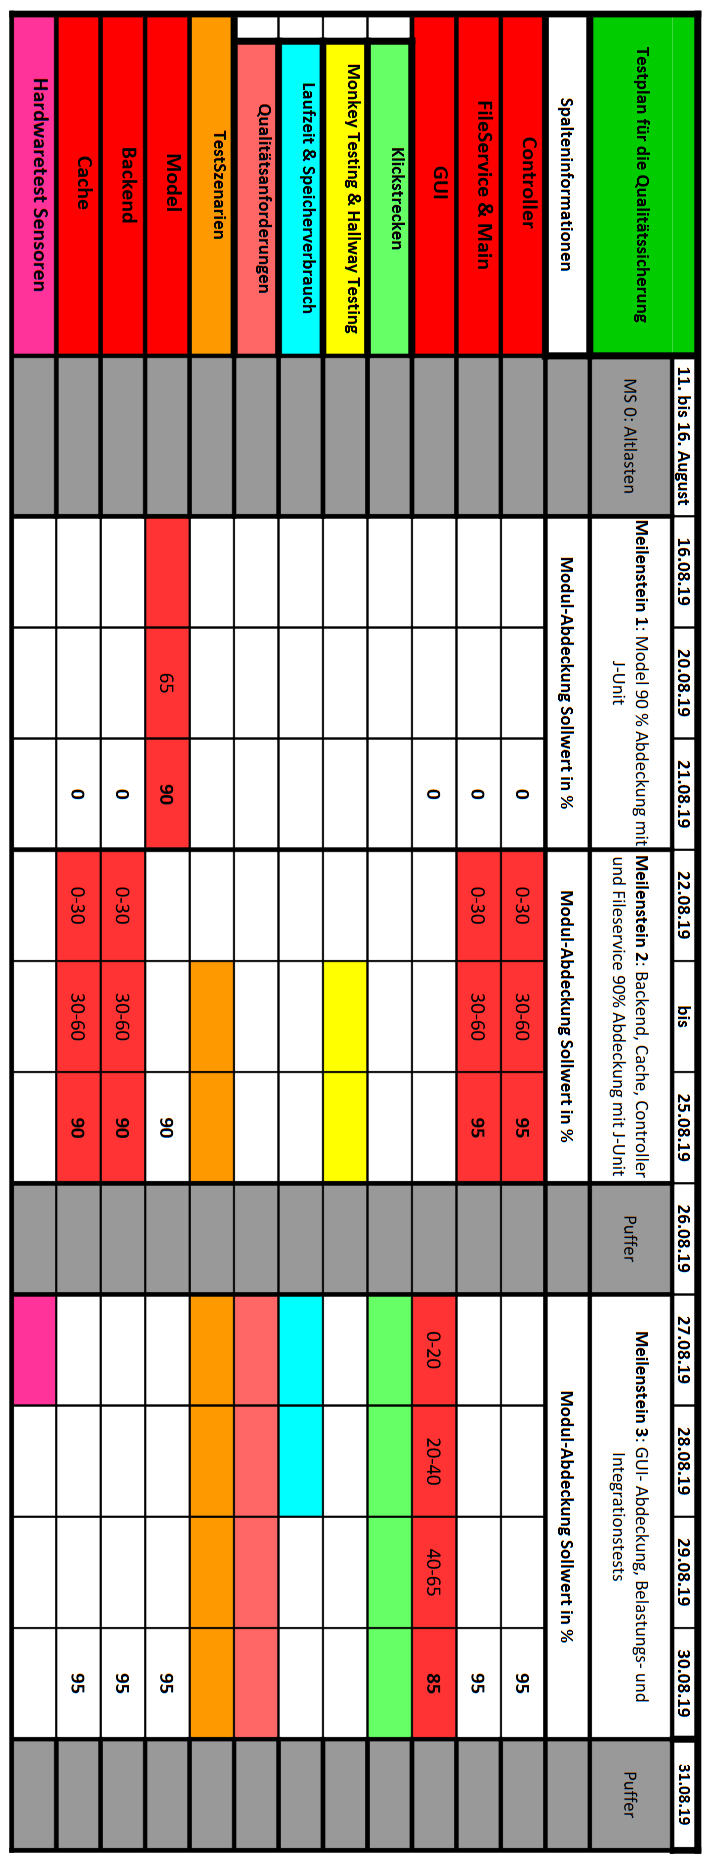
\includegraphics[width = 8cm]{Grafiken/sollplan.png}
		\caption{Der Sollpan für die Qualtätssicherungsphase.}
		\label{sollplan}
	\end{center}
\end{figure}


TODO: Wie ist der Plan am Ende der Phase aufgegangen?


\clearpage
\section{Gefundene Fehler und deren Regressionstests} \label{regression}

Dieses Kapitel umfasst die Regressionstests für gefundene und behobene Fehler. Die Tests sind nach Modul und Klassen strukturiert. Jeder Regressionstest verweist auf ein Issue der verwendeten Bugtracking-Software (hier GitHub).

\subsection{Übersicht aller Issues}
In der Tabelle \ref{issueOverView} wird angezeigt, wo ein Issue aufgetreten ist, und was für eine Kategorie es hat. Das Issue wird dabei durch seine Nummer repräsentiert. Zu den roten Issues gibt es keine Regressionstests, das diese nicht behoben wurden.

\begin{table}[h]
\begin{tabular}{| p{3cm} | p{2,2cm} | p{2,2cm}  |p{2,2cm} |p{2,2cm} |p{2,2cm}|}
	\hline
	\textbf{Art des Issue vs Fundort} & \textbf{Null Pointer} & \textbf{Index out Of Bounds} & \textbf{Path related} & \textbf{fehlerhafte Funktion} & \textbf{Sonstige} \\ \hline
	\textbf{Backend}
	& 
	
	&
	
	&
	
	&
	
	&
	36
	\\ \hline
	
	\textbf{Cache}
	& 
	
	&
		
	&
	&
	&
	\\ \hline
	
	\textbf{Controller}
	& 
	
	&

	&
	&
	&
	\\ \hline
	\textbf{Gui}
	& 
	27
	&
	&
	
	
	&
	15
	&
	\\ \hline
	
	\textbf{Model}
	& 
	7, 8, 9, 10, 12, 13, 19, 51, 59, 60
	&
	11, 18
	&	
	
	&
	21, 35
	&
	33, 53
	\\ \hline
	
	\textbf{Fileservice und Main}
	& 
	47
	&
	
	&
	57
	&
	50
	&
		
	\\ \hline

	\textbf{Gesamtzahl}
	& 
	&
	&
	&
	&
	\\ \hline
	
\end{tabular}
\caption{Übersicht über alle Issues.}
\label{issueOverView}
\end{table}

\clearpage
\subsection{Model}
\subsubsection{Measurement Configuration}

\begin{description}
 

\item []\textbf{Issue Nr.7 in der Methode getInChan} 

\begin{itemize}
\item []\textbf{Fehlersymptom:} Unbehandelte NullPointer Exception bei Eingabe einer ungültigen Id.
\item []\textbf{Fehlerursache:} Prüfen nach NullPointer Exception fehlt.
\item []\textbf{Fehlerbehebung:} Eine Null Prüfung wurde implementiert.
\item []\textbf{Verantwortlicher:} David Gawron
\end{itemize}

\item []\textbf{Issue Nr.8 in der Methode getOutChan} 

\begin{itemize}
\item []\textbf{Fehlersymptom:} Unbehandelte NullPointer Exception bei Eingabe einer ungültigen Id.
\item []\textbf{Fehlerursache:} Prüfen nach NullPointer Exception fehlt.
\item []\textbf{Fehlerbehebung:} Eine Null Prüfung wurde implementiert.
\item []\textbf{Verantwortlicher:} David Gawron
\end{itemize}

\item []\textbf{Issue Nr.9 in der Methode addConnection} 

\begin{itemize}
\item []\textbf{Fehlersymptom:} Unbehandelte NullPointer Exception bei Eingabe einer ungültigen Id.
\item []\textbf{Fehlerursache:} Prüfen nach NullPointer Exception fehlt.
\item []\textbf{Fehlerbehebung:} Eine Null Prüfung wurde implementiert.
\item []\textbf{Verantwortlicher:} David Gawron
\end{itemize}

\item []\textbf{Issue Nr.10 in der Methode removeConnection } 

\begin{itemize}
\item []\textbf{Fehlersymptom:} Unbehandelte NullPointer Exception bei Eingabe einer ungültigen Id.
\item []\textbf{Fehlerursache:} Prüfen nach NullPointer Exception fehlt.
\item []\textbf{Fehlerbehebung:} Eine Null Prüfung wurde implementiert.
\item []\textbf{Verantwortlicher:} David Gawron
\end{itemize}

\item []\textbf{Issue Nr.11 in der Methode createInChannelList } 

\begin{itemize}
\item []\textbf{Fehlersymptom:} Auftreten einer Index Out Of Bounds Exception.
\item []\textbf{Fehlerursache:} Eine Prüfung, ob der Index groß genug ist, fehlt.
\item []\textbf{Fehlerbehebung:} Der Fehler wird abgefangen durch einen Vergleich der Anzahl der InChannel zwischen yaml-File und Prototypblock.
\item []\textbf{Verantwortlicher:} David Gawron
\end{itemize}

\item []\textbf{Issue Nr.12 in der Methode getOutChanPosi } 

\begin{itemize}
\item []\textbf{Fehlersymptom:} NullPointer Exception beim Laden einer Messkonfiguration mit ungültigen Block Id.
\item []\textbf{Fehlerursache:} Prüfen nach NullPointer Exception fehlt.
\item []\textbf{Fehlerbehebung:} Es wird nach Null geprüft. Dann ergab sich eine Folgefehler, der sich in der Methode  createLoadedConnections als eine Index Out Of Bounds Exception äußerte. Durch das Implementieren einer Methode checkBlockInitId, die prüft, ob eine geladene Id auch gültig ist, wurde der Folgefehler behoben.
\item []\textbf{Verantwortlicher:} David Gawron
\end{itemize}


\item []\textbf{Issue Nr.13 in der Methode createInChannelList } 

\begin{itemize}
\item []\textbf{Fehlersymptom:} NullPointer Exception bei ungültiger Messkonfiguration mit einer fehlenden BlockChannelliste.
\item []\textbf{Fehlerursache:} Prüfen nach NullPointer Exception fehlt.
\item []\textbf{Fehlerbehebung:} Eine Prüfung nach Null wurde hinzugefügt.
\item []\textbf{Verantwortlicher:} David Gawron
\end{itemize}


\item []\textbf{Issue Nr.14 in der Methode loadConfig} 

\begin{itemize}
\item []\textbf{Fehlersymptom:} Fehlerhaftes Verhalten beim Laden der fehlerhaften Messkonfiguration 4, die einen Block mit sich selber verbindet.
\item []\textbf{Fehlerursache:} Überprüfen der Verbindung fehlt.
\item []\textbf{Fehlerbehebung:} Die Überprüfung der Verbindung wurde implementiert.
\item []\textbf{Verantwortlicher:} David Gawron
\end{itemize}

\item []\textbf{Issue Nr.18 in der Methode removeBlock} 

\begin{itemize}
\item []\textbf{Fehlersymptom:} Der Versuch einen nicht existierenden Block zu entfernen, resultiert in eines Index Out Of Bounds Exception.
\item []\textbf{Fehlerursache:} Der Index wurde nicht geprüft.
\item []\textbf{Fehlerbehebung:} Eine Prüfung des Indexes wurde hinzugefügt. Außerdem wurde der Rückgabewert der Methode von void zu boolean geändert.
\item []\textbf{Verantwortlicher:} David Gawron
\end{itemize}

\item []\textbf{Issue Nr.19 in der Methode removeBlock} 

\begin{itemize}
\item []\textbf{Fehlersymptom:} Der Versuch eine Konfiguration ohne eine Liste von Block Ids zu laden, führt zu einer Null Pointer Exception.
\item []\textbf{Fehlerursache:} Es wurde nicht nach Null geprüft.
\item []\textbf{Fehlerbehebung:} Die betreffende Zeile wurde in einen schon existierenden Null-Check verschoben.
\item []\textbf{Verantwortlicher:} David Gawron
\end{itemize}

\item []\textbf{Issue Nr.23 in der Methode loadConfig} 

\begin{itemize}
\item []\textbf{Fehlersymptom:} Der Versuch eine Konfiguration mit einem Splitter mit vertauschten Verbindungstupel führt zu einem ungewollten Fehlschlag des Ladens.
\item []\textbf{Fehlerursache:} Die private Methode createInChannelList, die von loadConfig benutzt wird, funktionierte nicht korrekt.
\item []\textbf{Fehlerbehebung:} Die private Methode createInChannelList wurde reimplementiert.
\item []\textbf{Verantwortlicher:} David Gawron
\end{itemize}


\item []\textbf{Fehler Nr.35 in der Methode getInitId} 

\begin{itemize}
\item []\textbf{Fehlersymptom:} Die Methode funktionierte nicht richtig und gab immer NULL zurück.
\item []\textbf{Fehlerursache:} Der Zugriff auf die Blöcke in der Hasmap der Konfigurationsblöcke schlägt fehl.
\item []\textbf{Fehlerbehebung:} Die KonfigurationsId wird nun über die Blockliste der Messkonfiguration geholt.
\item []\textbf{Verantwortlicher:} David Gawron
\end{itemize}

\end{description}

\subsubsection{Sensor}

\begin{description}

\item []\textbf{Issue Nr.51 in der Methode constructBuildingBlocks} 

\begin{itemize}
\item []\textbf{Fehlersymptom:} Die Methode liefert bei Übergabe von null oder einer leeren Map eine NullPointerException.
\item []\textbf{Fehlerursache:} Fehlende Überprüfung der Übergabewerte auf die notwendigen Argumente
\item []\textbf{Fehlerbehebung:} constructBuildingBlock() überprüft, ob die Map null oder leer ist.
\item []\textbf{Verantwortlicher:} Linus Ruhnke
\end{itemize}

\item []\textbf{Issue Nr.59 in der Methode processKvPair} 

\begin{itemize}
\item []\textbf{Fehlersymptom:} Die Methode liefert bei falschen Übergabewerten eine NullPointerException.
\item []\textbf{Fehlerursache:} Fehlende Überprüfung der Übergabewerte auf die notwendigen Argumente
\item []\textbf{Fehlerbehebung:} processKvPair() überprüft, ob die Map der Bausteine die notwendigen Argumente zum Aufbauen des Bausteins enthält. 
\item []\textbf{Verantwortlicher:} Linus Ruhnke
\end{itemize}

\item []\textbf{Issue Nr.60 in der Methode initialiseModel} 

\begin{itemize}
\item []\textbf{Fehlersymptom:} Die Methode überprüft Bausteine nicht auf null und kann somit eine NullPointerException liefern.
\item []\textbf{Fehlerursache:} Fehlende Überprüfung der Bausteine auf die null.
\item []\textbf{Fehlerbehebung:} Die Methode überprüft, ob die Bausteine null sind.
\item []\textbf{Verantwortlicher:} Linus Ruhnke
\end{itemize}

\end{description}

\subsubsection{BuildingBlockDirectory}

\begin{description}

\item []\textbf{Issue Nr.21 in der Methode addConfigBlock} 

\begin{itemize}
\item []\textbf{Fehlersymptom:} Konfigurationsbausteine konnten mehrfach mit dem gleichen Key zu der Liste hinzugefügt werden. Alte Einträge mit dem gleichen Key wurden überschrieben.
\item []\textbf{Fehlerursache:} Standart-Funktion einer HashMap.
\item []\textbf{Fehlerbehebung:} Konfigurationsbausteine können nicht mehrfach mit dem gleichen Key hinzugefügt werden. Alte Einträge werden nicht mehr überschrieben.
\item []\textbf{Verantwortlicher:} Linus Ruhnke
\end{itemize}

\end{description}


\clearpage
\subsection{Cache}



\clearpage
\subsection{Backend}

\begin{description}

\item []\textbf{Issue Nr.36 in der Klasse PickupPointForBackendAgents} 

\begin{itemize}
\item []\textbf{Fehlersymptom:} Es war nicht möglich, gleichzeitig eine simulierte und eine tatsächliche Backend-Verbindung aufzubauen.
\item []\textbf{Fehlerursache:} Durch PickupPointForBackendAgents wurde immer nur entweder eine echte oder eine simulierte Verbindung initialisiert.
\item []\textbf{Fehlerbehebung:} Durch separate Methoden können nun eine echte und eine simulierte Verbindung separat verwendet werden.
\item []\textbf{Verantwortlicher:} Jan Küblbeck
\end{itemize}

\end{description}


\clearpage
\subsection{Controller}



\clearpage
\subsection{Fileservice und Main}

\begin{description}

\item []\textbf{Issue Nr.47 in der Methode readOutAllYamll} 

\begin{itemize}
\item []\textbf{Fehlersymptom:} Bei einem Fehler beim Lesen des Inhalt einer Yaml-Datei wird null zurückgegeben.
\item []\textbf{Fehlerursache:} Implementierung der Methode.
\item []\textbf{Fehlerbehebung:} Bei einem Fehler beim Lesen wird eine leere Map zurückgegeben.
\item []\textbf{Verantwortlicher:} Linus Ruhnke
\end{itemize}

\item []\textbf{Issue Nr.50 in der Methode testWriteIntoYaml} 

\begin{itemize}
\item []\textbf{Fehlersymptom:} Die Methode löschte eine durch den Test erzeugte Methode bei einem erfolgreichen Durchlauf nicht, was zur Folge hatte, dass beim nächsten Test der Test fehl schlug.
\item []\textbf{Fehlerursache:} Unbekannt.
\item []\textbf{Fehlerbehebung:} Die Methode löscht vor dem Test die Datei aus dem Verzeichniss.
\item []\textbf{Verantwortlicher:} Linus Ruhnke
\end{itemize}

\item []\textbf{Issue Nr.57 in der Methode readFromYaml} 

\begin{itemize}
\item []\textbf{Fehlersymptom:} Falls ein angegebener Pfad nicht existiert wird eine Exception von SnakeYaml übergeben.
\item []\textbf{Fehlerursache:} Übergebener Pfad existiert nicht, aber wird nicht abgefangen.
\item []\textbf{Fehlerbehebung:} Vor dem Lesen wird überprüft, ob eine Ressource in dem Verzeichnis mit dem Pfad existiert.
\item []\textbf{Verantwortlicher:} Linus Ruhnke
\end{itemize}

\end{description}


\clearpage
\subsection{GUI}

\begin{description}

\item []\textbf{Issue Nr.27 in der Methode pushData} 

\begin{itemize}
\item []\textbf{Fehlersymptom:} NullPointerException tritt auf, wenn ein Messlauf begonnen wird ohne zuvor die GUI zu starten.
\item []\textbf{Fehlerursache:} Es wurde in der Klasse DataVisualisation auf ein Textfeld zugegriffen, welches nicht initialisiert wurde.
\item []\textbf{Fehlerbehebung:} Das Textfeld wird nun zuerst auf null überprüft.
\item []\textbf{Verantwortlicher:} Jan Küblbeck
\end{itemize}

\end{description}


\clearpage
\section{Testen der GUI} \label{gui}


\subsection{Testen der GUI durch Klickstrecken}

\subsubsection{Öffnen der Systemmenüs und dessen Funktionen}

In dieser Klickstrecke werden die Funktionen des Systemleistenmenüs getestet unter der Vorbedinung, dass die Anwendung geöffnet ist. In Klickstrecke Nr.1 werden mehrere Bausteine bei der Initialisierung der Anwendung geladen und bei Klickstrecke Nr.2 sind keine Bausteine bei dem angegeben Pfad initialisiert worden. 

\begin{table}[h]
\begin{tabular}{| p{0,5cm} | p{6,5cm} | p{3,5cm} | p{3,5cm} |}
	\hline
	\textbf{Nr.} & \textbf{Aktions- und Klickstrecke} & \textbf{Erwartetes Ergbenis}  & \textbf{ Bewertung tatsächliches Ergebnis} \\ \hline
	\textbf{1}
	& 
	Anwendung wird geöffnet $\rightarrow$ Systemmenü "Bausteine" wird gedrückt.
	&
	"Prototyp-Bausteine" - Fenster wird geöffnet. Geladene Bausteine werden im dem Fenster angezeigt.
	& 
	Das erwartete Ergebnis stimmt mit dem dem tatsächlichen Ergebnis überein.
	\\ \hline
	
	\textbf{2}
	& 
	Anwendung wird geöffnet $\rightarrow$ Systemmenü "Bausteine" wird gedrückt.
	&
	"Prototyp-Bausteine" - Fenster wird geöffnet. Es werden keine Bausteine im Fenster angezeigt
	& 
	Das erwartete Ergebnis stimmt mit dem dem tatsächlichen Ergebnis überein.
	\\ \hline
	
	\textbf{3}
	& 
	Systemmenü "Bausteine" wird gedrückt $\rightarrow$ Sensoren-Untermenü wird geöffnet $\rightarrow$ Transformation-Untermenü wird geöffnet $\rightarrow$ Repräsentation-Untermenü wird geöffnet.
	&
	Beim Öffnen der Untermenüs werden die einzelnen Bausteine der unterschiedlichen Typen angezeigt.
	& 
	Das erwartete Ergebnis stimmt mit dem dem tatsächlichen Ergebnis überein.
	\\ \hline



	\textbf{4}
	& 
	Klicke auf "Bearbeiten" Knopf unter den Namen der Bausteine $\rightarrow$ Bearbeiten der Baustein-Informationen durch 
	Editieren des Textfeldes der Wert- Spalte.
	&
	Beim Drücken des Knopfes öffnet sich das "Eigenschaften" Fenster mit Baustein-Spezifischen Informationen über den 				Baustein. Eigenschaften lassen sich bearbeiten und der dadurch neu entstandene Baustein soll gespeichert oder weiterverwendet werden können.
	& 
	Es öffnet sich das "Einstellungen" Fenster im Hintergrund hinter dem "Prototyp-Bausteine" Fenster. Es werden nicht alle 			Eigenschaften, welche in der Tabelle dargestellt werden sollen dargestellt. Das Wert-Textfeld lässt sich editieren. Das				Editieren des Textfeld erfüllt jedoch keine Funktionalität und lässt keine weiteren Funktionalitäten zu.
	\\ \hline
	
	\textbf{5}
	& 
	Systemmenü "Einstellungen" wird gedrückt.
	&
	Es öffnet sich das "Einstellungen" Fenster im Vordergrund der Anwendung, bestehend aus mehreren Untermenüs zu 				verschiedenen Einstellungsmöglichkeiten.
	& 
	Das erwartete Ergebnis stimmt mit dem dem tatsächlichen Ergebnis überein.
	(Weitere Klickstrecken zum "Einstellungen" Menü im Unterpunkt 4.1.todo)
	\\ \hline

	\end{tabular}
	\end{table} 


	\begin{table}[h]
\begin{tabular}{| p{0,5cm} | p{6,5cm} | p{3,5cm} | p{3,5cm} |}
	\hline
	\textbf{Nr.} & \textbf{Aktions- und Klickstrecke} & \textbf{Erwartetes Ergebnis}  & \textbf{ Bewertung tatsächliches Ergebnis} \\ \hline

	\textbf{6}
	& 
	Systemmenü "Hilfe" wird gedrückt.
	&
	Es öffnet sich das "Hilfe" Fenster im Vordergrund der Anwendung. In diesem Fenster sind Informationen über die 				Anwendung, wie auch über die Entwicklung zu finden. Zu den wichtigesten Funktionen der Anwendung gibt es ebenfalls 			kleinere Tutorials.
	& 
	Das erwartete Ergebnis stimmt mit dem dem tatsächlichen Ergebnis überein.
	\\ \hline

	\textbf{7}
	& 
	
	&
	
	& 
	
	\\ \hline

	\textbf{8}
	& 
	
	&
	
	& 
	
	\\ \hline

	\textbf{9}
	& 
	
	&
	
	& 
	
	\\ \hline
	
\end{tabular}
\caption{Testen der Systemmenüs und dessen Funktionen.}
\label{klickMenu}
\end{table} 

\subsubsection{Erstellen, Speichern und Laden einer Messkonfiguration}

In dieser Klickstrecke wird die Anwendung anhand ihrer Funktion rund um das Erstellen, Speichern und Laden einer Messkonfiguration getestet. Als Vorbedingung ist hier die geöffnete Anwendung mit einer leeren Messkonfiguration gegeben. Die Klickstrecke und deren Ergebnisse sind in Tabelle \ref{klickConfig} zu sehen. Dabei besteht Konfiguration A aus einem BMP180 Sensor-Baustein, einer textuellen Repräsentation für einen Kanal und der korrekten Verbindung dazwischen. Konfiguration B besteht aus dem selben Bausteinen wie Konfiguration A, aber die Verbindung fehlt.  

\begin{table}[h]
\begin{tabular}{| p{0,5cm} | p{6,5cm} | p{3,5cm} | p{3,5cm} |}
	\hline
	\textbf{Nr.} & \textbf{Aktions- und Klickstrecke} & \textbf{Erwartetes Ergebnis}  & \textbf{ Bewertung tatsächliches Ergebnis} \\ \hline
	\textbf{1}
	& 
	Erstelle Konfiguration A $\rightarrow$ klicke auf Check-Knopf $\rightarrow$ klicke auf Ok $\rightarrow$ klicke auf Speichern-Knopf $\rightarrow$ wähle Namen und Pfad aus und klicke auf Speichern 
	&
	Die Datei mit dem entsprechenden Namen ist am entsprechenden Ort zu finden. Die Datei enthält die Konfiguration A.
	& 
	to do
	\\ \hline
	
	\textbf{2}
	& 
	Erstelle Konfiguration B $\rightarrow$ klicke auf Check-Knopf
	&
	Eine Meldung öffnet sich, dass die Konfiguration nicht gültig ist.
	& 
	 TODO Das Ergebnis stimmt nicht überein, da ein Check-Knopf (noch) nicht existiert.
	\\ \hline
	
	\textbf{3}
	& 
	klicke auf Speichern-Knopf $\rightarrow$ klicke auf Abbrechen
	&
	Das Hauptfenster ist geöffnet und es hat sich nichts verändert.
	& 
	Das tatsächliche Ergebnis stimmt mit dem erwarteten Ergebnis überein.
	\\ \hline
	
	\textbf{4}
	& 
	klicke auf Laden-Knopf $\rightarrow$ klicke auf Abbrechen
	&
	Das Hauptfenster ist geöffnet und es hat sich nichts verändert.
	& 
	Das tatsächliche Ergebnis stimmt mit dem erwarteten Ergebnis überein.
	\\ \hline
	
	\textbf{5}
	& 
	klicke auf Laden-Knopf $\rightarrow$ klicke auf laden, wobei Konfiguration A aus Nr. 1 ausgewählt ist
	&
	Eine Fenster öffnet sich und zeigt an, dass die Konfiguration erfolgreich geladen wurde.
	& 
	Das tatsächliche Ergebnis stimmt mit dem erwarteten Ergebnis überein.
	\\ \hline
	\textbf{6}
	& 
	klicke auf Laden-Knopf $\rightarrow$ klicke auf laden, wobei Konfiguration B aus Nr. 2 ausgewählt ist
	&
	Eine Fenster öffnet sich und zeigt an, dass die Konfiguration nicht gültig, und somit nicht startbar ist.
	& 
	Das tatsächliche Ergebnis stimmt mit dem erwarteten Ergebnis überein.
	\\ \hline
		
	
	
\end{tabular}

\caption{Klickstrecke um das Erstellen, Laden und Speichern einer Messkonfiguration mit der Gui zu testen.}
\label{klickConfig}
\end{table}

\subsubsection{Kontrolle des Messlaufs}

Durch diese Klickstrecke (Tabelle \ref{klickMesslauf}) wird überprüft, ob das Starten, Pausieren, Fortsetzen und Beenden eines Messlaufs und das Speichern von Messdaten korrekt funktioniert. Vorbedingung: die Messkonfiguration ist bereits geladen (siehe vorherige Klickstrecke)

\begin{table}[h]
\begin{tabular}{| p{0,5cm} | p{6,5cm} | p{3,5cm} | p{3,5cm} |}
	\hline
	\textbf{Nr.} & \textbf{Aktions- und Klickstrecke} & \textbf{Erwartetes Ergebnis}  & \textbf{ Bewertung tatsächliches Ergebnis} \\ \hline
	\textbf{1}
	& 
	klicke ``Run Configuration''
	&
	Auslesen und Anzeigen der Messdaten (Messlauf) beginnt
	& 
	Das tatsächliche Ergebnis stimmt mit dem erwarteten Ergebnis überein.
	\\ \hline
	
	\textbf{2}
	& 
	klicke ``Pause''
	&
	Es werden keine neuen Daten verarbeitet und angezeigt.
	& 
	Das tatsächliche Ergebnis stimmt mit dem erwarteten Ergebnis überein.
	\\ \hline
	
	\textbf{3}
	& 
	klicke ``Resume''
	&
	Der Messlauf wird fortgesetzt.
	& 
	Das tatsächliche Ergebnis stimmt mit dem erwarteten Ergebnis überein.
	\\ \hline
	
	\textbf{4}
	& 
	klicke ``Pause'' $\rightarrow$ ``Save Measurement Data'' $\rightarrow$ wähle Zielpfad aus $\rightarrow$ klicke ``Save''
	&
	bisher gemessene Daten werden in einer Datei gespeichert
	& 
	Das tatsächliche Ergebnis stimmt mit dem erwarteten Ergebnis überein.
	\\ \hline
	
	\textbf{5}
	& 
	klicke ``Reset''
	&
	Der Messlauf wird auf den ursprünglichen Zustand zurückgesetzt.
	& 
	Die angezeigten Messdaten werden nicht aus dem Anzeigefeld entfernt.
	\\ \hline
	
\end{tabular}

\caption{Kontrolle des Messlaufs}
\label{klickMesslauf}
\end{table}

\subsection{Monkey Testing}

\clearpage
\section{Testen der Qualität} \label{quali}



\subsection{Hallway Usability Testing}


\subsection{Testen der Qualität der Funktionalitäten}



\section{Durchführen der Testfälle aus dem Pflichtenheft} \label{testszenarien}

\subsection{\textbf{T010} Starten der Anwendung und Hilfe}

DISCLAIMER: Der Testfall wurde so nicht wirklich durchgeführt, da der Pfad zur Textdatei noch nicht richtig funktioniert. Siehe Issue Nr. 15 in Git-Hub. Der Testfall wurde so angelegt, wie er später aussehen könnte. Er dient lediglich dazu, frühzeitig Feedback zu erhalten.

\begin{table}[h]
\begin{tabular}{| p{4cm} | p{10cm} |}
	\hline
	\textbf{Strukturelement} & \textbf{Beschreibung} \\ \hline
	\textbf{Testfallnummer (Pflichtenheft)}
	& 
	T10
	\\ \hline
	
	\textbf{Testfallverweis}
	& 
	hat ein Testfall vom Pflichtenheft eine JUnit-Test-Datei mit ein oder mehreren Tests?
	\\ \hline
	
	\textbf{(optional) Subunittests}
	& 
	\\ \hline
	
	\textbf{Verantwortlicher Tester}
	& 
	David
	\\ \hline
	
	
	\textbf{Vorbedingung}
	& 
	Die Anwendung ist als fat-Jar-Datei auf dem Rechner vorhanden. Es läuft keine Instanz dieser Anwendung.
	\\ \hline
	
	\textbf{ Testziel}
	& 
	Zu Testen ist das Verhalten des Anwendung, wenn sie gestartet wird. Außerdem soll die Hilfe-Funktion der Anwendung getestet werden.
	\\ \hline
	
	
	\textbf{Beschreibung}
	& 
	Die Anwendung öffnet sich bei dem Öffnen der fat-Jar-Datei. Dabei öffnet sich das Hauptfenster, in dem keine Messkonfiguration zu sehen ist. Drückt man den Knopf für die Hilfe, öffnet sich das Hilfefenster mit Informationen über die Benutzung der Anwendung.
	\\ \hline
	
	\textbf{Erwartetes Ergebnis}
	& 
	Das Hauptfenster und das Hilfefenster öffnen sich wie gewollt.
	\\ \hline
			
	\textbf{Verhalten im Fehlerfall}
	& 
	Eine Fehlermeldung wird angezeigt, falls beim Pfad zur Textdatei für das Hilfefenster keine Datei gefunden wurde.
	\\ \hline
	
	\textbf{Nachbedingung}
	& 
	Das Hauptfenster der Anwendung ist geöffnet. Es wird von dem geöffneten Hilfe-Fenster teilweise überdeckt.
	\\ \hline
	
	
	\textbf{Getestete Anforderungen}
	& 
	\textbf{F010} erreiche GUI nach Start, \textbf{F140} leere Darstellung nach Anwendungsstart, \textbf{F480} Hilfe zu Anwendung, \textbf{F490} Texte der Anwendung auf Deutsch
	\\ \hline
	
	
	
\end{tabular}
\caption{Testfall T10 aus dem Plfichtenheft: Öffnen der Anwendung und Hilfe.}
\label{testfallT10}
\end{table}




\subsection{\textbf{T020} Starten der Demo}



\subsection{\textbf{T030} Lehrer erstellt und speichert eine Messkonfiguration}
Die Durchführung dieses Testfalles ist in Tabelle \ref{testfallT30} zu sehen. Der Testfall aus dem Pflichtenheft schlägt fehl, weil viele Features nicht oder nur teilweise implementiert sind.


\begin{table}[h]
\begin{tabular}{| p{4cm} | p{10cm} |}
	\hline
	\textbf{Strukturelement} & \textbf{Beschreibung} \\ \hline
	\textbf{Testfallnummer (Pflichtenheft)}
	& 
	T30
	\\ \hline
	\textbf{Verantwortlicher Tester}
	& 
	David
	\\ \hline
	\textbf{Vorbedingung}
	& 
	Die Anwendung ist geöffnet, das Konfigurationsfeld ist leer.
	\\ \hline
	\textbf{ Testziel}
	& 
	Zu Testen ist das Verhalten des Anwendung, wenn eine Konfiguration über den Editor teilweise erstellt wird, und als Zwischenergebnis gespeichert wird.
	\\ \hline
	
	\textbf{Klickstrecke}
	& 
	erstelle Konfiguration (siehe Beschreibung) $\rightarrow$ klicke auf Speichern-Knopf $\rightarrow$ wähle Pfad und Namen aus und klicke auf speichern
	\\ \hline
	
	\textbf{ Beschreibung}
	& 
	Der Benutzer erstellt eine Konfiguration textuell über den Editor. Dabei gibt er die Blöcke als Liste von BlockIds an. Hier enthält die Liste zwei Sensoren(BMP180, MMA8451) und eine Transformation(Transformation-Add-2-Channel). Zu den drei Bausteinen erstellt der Benutzer eine jeweilige List ihrer Channel. Die Liste aller Verbindungen bleibt hier leer.
	\\ \hline
	
	\textbf{Abweichungen vom Pflichtenheft}
	& 
	Der Ablauf dieses Testfalles unterscheidet sich massiv von dem Testfall aus dem Pflichtenheft. Die Anwendung unterstützt kein Drag-and-Drop. Deshalb kann auch kein Baustein im Konfigurationsfeld als Icon sichtbar werden. Hier erfolgt die Erstellung der Konfiguration ausschließlich textuell über den Editor. Außerdem prüft die Anwendung nicht, ob der entsprechende Sensor angeschlossen ist, wenn ein Sensorbaustein hinzugefügt wird. Weiter überprüft die Anwendung nicht explizit beim Speichern, ob die Messkonfiguration gültig oder vollständig ist. Dies geschieht entweder über den Check-Knopf oder beim Laden der Konfiguration. Es könne keine expliziten Einstellung für nur eine Messkonfiguration eingestellt und mit ihr gespeichert werden. 

	\\ \hline
	
	\textbf{Erwartetes Ergebnis}
	& 
	Die Anwendung ist geöffnet, die Konfiguration ist im Konfigurationsfeld zu sehen. Außerdem ist ein Fenster geöffnet, mit der Meldung, dass die Konfiguration erfolgreich gespeichert wurde.	Die unfertige Konfiguration ist als Datei am entsprechenden Ort als Datei gespeichert. 
	\\ \hline
			
	\textbf{Verhalten im Fehlerfall}
	& 
	Die Anwendung gibt nur bei Benutzung des Check-Knopfes an, ob die Konfiguration gültig ist.
	\\ \hline
	
	\textbf{Nachbedingung}
	& 
	Das Hauptfenster der Anwendung ist geöffnet. Es wird von dem geöffneten Hilfe-Fenster teilweise überdeckt.
	\\ \hline
	
	
	\textbf{Getestete Anforderungen}
	& 
	\textbf{F180} füge Sensor hinzu, \textbf{F210} füge Transformation hinzu, \textbf{F250} speichere Messkonfiguration
	\\ \hline
	\textbf{fehlende zu testete Anforderungen}
	& 
	\textbf{F190} prüfe ob Sensor angeschlossen, \textbf{F290} Einstellungen Messkonfiguration 
	\\ \hline
	
	
\end{tabular}
\caption{Testfall T30 aus dem Plfichtenheft: Öffnen der Anwendung und Hilfe.}
\label{testfallT30}
\end{table}



\subsection{\textbf{T040} Schüler bearbeitet Aufgabe}

Die Durchführung dieses Testfalles ist in Tabelle \ref{testfallT40} zu sehen. Dabei wird bei dem Informieren über die Bausteine das Untermenü aller Bausteine beliebig genutzt. Eine explizite Klickstrecke wird nicht angegeben, da eine solche über alle Bausteine viel Schreibarbeit und wenig Erkenntnis bringt


\begin{table}[h]
\begin{tabular}{| p{4cm} | p{10cm} |}
	\hline
	\textbf{Strukturelement} & \textbf{Beschreibung} \\ \hline
	\textbf{Testfallnummer (Pflichtenheft)}
	& 
	T40
	\\ \hline
	\textbf{Verantwortlicher Tester}
	& 
	David
	\\ \hline
	\textbf{Vorbedingung}
	& 
	Die Anwendung ist geöffnet, das Konfigurationsfeld ist leer.
	\\ \hline
	\textbf{ Testziel}
	& 
	Zu Testen ist das Laden einer unvollständigen Konfiguration, deren Vervollständigung und das speichern der kompletten Konfiguration.
	\\ \hline
	
	\textbf{Klickstrecke}
	& 
	klicke auf Laden-Knopf $\rightarrow$ wähle richtige Datei aus und klicke auf laden $\rightarrow$ klicke auf OK $\rightarrow$ klicke auf Bausteine in der Systemleiste und informiere dich $\rightarrow$ klicke auf X $\rightarrow$ klicke auf Hilfe und informiere dich klicke auf X $\rightarrow$ vervollständige Konfiguration und klicke auf Check-Knopf $\rightarrow$ klicke Meldung(Konfiguration gültig) weg $\rightarrow$ klicke auf speichern und führe den Dialog korrekt aus
	\\ \hline
	
	\textbf{ Beschreibung}
	& 
	Die ungültige Konfiguration wird geladen. Die Angebotenen Bausteine sind im Untermenü der Bausteine zu finden. Der Benutzer bearbeitet die Konfiguration, in dem er der Liste eine textuelle Repräsentation mit drei Kanälen hinzufügt. Außerdem erstellt er die Liste der Verbindungen. Eine Verbindung ist dabei ein Tupel zweier Kanäle. Ist der Benutzer der Meinung, dass die Konfiguration fertig ist, kann er den Check-Knopf benutzten, um zu prüfen, ob die Konfiguration gültig ist. Die Konfiguration kann jederzeit gespeichert und geladen werden.
	\\ \hline
	
	\textbf{Abweichungen vom Pflichtenheft}
	& 
	Die Anwendung prüft nicht beim Laden der Konfiguration, ob für die benutzten Sensorbausteine entsprechende Sensoren angeschlossen sind. Außerdem kann die Anwendung die graphische Darstellung der Konfiguration nicht aktualisieren, dass es keine solche gibt.

	\\ \hline
	
	\textbf{Erwartetes Ergebnis}
	& 
	Die vollständige Konfiguration ist als Datei am entsprechenden Pfad zu finden.
	\\ \hline
			
	\textbf{Verhalten im Fehlerfall}
	& 
	Beim Laden gibt die Anwendung an, dass die Konfiguration ungültig ist und bearbeitet werden sollte. Außerdem gibt sie bei Benutzung des Check-Knopfes an, ob die Konfiguration gültig ist.
	\\ \hline
	
	\textbf{Nachbedingung}
	& 
	Das Hauptfenster der Anwendung ist geöffnet. Die vollständige Konfiguration ist im Feld zu sehen.  Sie ist auch als Datei gespeichert.
	\\ \hline
	
	
	\textbf{Getestete Anforderungen}
	& 
	\textbf{F230} füge Darstellung hinzu, \textbf{F470} Hilfe zu Bausteinen
	\\ \hline
	\textbf{fehlende zu testete Anforderungen}
	& 
	
	\\ \hline
	
	
\end{tabular}
\caption{Testfall T40 aus dem Plfichtenheft: Öffnen der Anwendung und Hilfe.}
\label{testfallT40}
\end{table}

\subsection{\textbf{T050} Schüler startet Messung und speichert Ergebnisse}

Die Durchführung dieses Testfalles ist in Tabelle \ref{testfallT050} zu sehen.

\begin{table}[h]
\begin{tabular}{| p{4cm} | p{10cm} |}
	\hline
	\textbf{Strukturelement} & \textbf{Beschreibung} \\ \hline
	\textbf{Testfallnummer (Pflichtenheft)}
	& 
	T050
	\\ \hline
	\textbf{Verantwortlicher Tester}
	& 
	Jan
	\\ \hline
	\textbf{Vorbedingung}
	& 
	Die Anwendung ist gestartet und es ist die in T040 erstelle Messkonfiguration geladen worden.
	\\ \hline
	\textbf{ Testziel}
	& 
	Teste die Anwendung aus Sicht eines Schülers, der Messung starten und deren Ergebnisse speichern soll.
	\\ \hline
	
	\textbf{Klickstrecke}
	& 
	klicke auf ``Run Configuration'' $\rightarrow$ warte, bis Daten angezeigt werden $\rightarrow$ klicke auf ``Pause'' $\rightarrow$ klicke auf ``Save Measurement Data'' $\rightarrow$ definiere, wo die Daten gespeichert werden sollen $\rightarrow$ klicke auf ``Save''
	\\ \hline
	
	\textbf{ Beschreibung}
	& 
	Der Messlauf, der durch die bereits vorbereitete Konfiguration definiert ist, wird gestartet. Nachdem einige Daten erfolgreich ausgelesen wurden, wird der Messlauf angehalten und die Daten gespeichert.
	\\ \hline
	
	\textbf{Abweichungen vom Pflichtenheft}
	& 
	Da die Daten in der umgesetzten Anwendung nicht grafisch dargestellt werden können, kann auch keine grafische Darstellung gespeichert werden.

	\\ \hline
	
	\textbf{Erwartetes Ergebnis}
	& 
	Die ausgelesenen Daten sind in einer Datei am angegebenen Pfad gespeichert.
	\\ \hline
			
	\textbf{Verhalten im Fehlerfall}
	& 
	Falls die Zieldatei bereits existiert, werden die Daten nicht gespeichert.
	\\ \hline
	
	\textbf{Nachbedingung}
	& 
	Das Hauptfenster der Anwendung ist geöffnet. Die Konfiguration ist weiterhin geladen. Der Messlauf ist im pausierten Zustand. Die bislang ausgelesenen Daten sind in einer Datei gespeichert.
	\\ \hline
	
	
	\textbf{Getestete Anforderungen}
	& 
	\textbf{F130, F300} Messung starten, \textbf{F150, F320} Messdaten werden angezeigt, \textbf{F370} Messung pausieren, \textbf{400} Messdaten speichern
	\\ \hline
	\textbf{fehlende zu testete Anforderungen}
	& 
	\textbf{F410} da kein Graph erzeugt wird, kann auch kein Graph gespeichert werden
	
	\\ \hline
	
	
\end{tabular}
\caption{Testfall T050 aus dem Plfichtenheft: Öffnen der Anwendung und Hilfe.}
\label{testfallT050}
\end{table}

\subsection{\textbf{T200} Laden einer ungültigen Datei als Messkonfiguration}

\subsection{\textbf{T210} Starten einer ungültigen Messkonfiguration}

\subsection{\textbf{T220} Entfernen eines Sensors bei laufender Messung}

Die Durchführung dieses Testfalles ist in Tabelle \ref{testfallT220} zu sehen.

\begin{table}[h]
\begin{tabular}{| p{4cm} | p{10cm} |}
	\hline
	\textbf{Strukturelement} & \textbf{Beschreibung} \\ \hline
	\textbf{Testfallnummer (Pflichtenheft)}
	& 
	T220
	\\ \hline
	\textbf{Verantwortlicher Tester}
	& 
	Jan
	\\ \hline
	\textbf{Vorbedingung}
	& 
	Die Anwendung ist geöffnet. Alle verwendeten Sensoren sind angeschlossen und betriebsbereit. Eine gültige Messkonfiguration aus zwei Sensoren, einer Transformation und einer Darstellung wurde geladen.
	\\ \hline
	\textbf{ Testziel}
	& 
	Teste das Verhalten der Anwendung, wenn ein Sensor ausfällt und dessen Datenstrom abbricht.
	\\ \hline
	
	\textbf{Klickstrecke}
	& 
	klicke auf ``Run Configuration'' $\rightarrow$ trenne Verbindung zum Sensor
	\\ \hline
	
	\textbf{ Beschreibung}
	& 
	Der Benutzer startet die Messung. Die Verbindung zu einem Sensor wird getrennt.
	\\ \hline
	
	\textbf{Abweichungen vom Pflichtenheft}
	& 
	

	\\ \hline
	
	\textbf{Erwartetes Ergebnis}
	& 
	Die Anwendung erkennt, dass ein Sensor keine Daten mehr sendet. Die Messung stoppt. Eine aussagekräftige Fehlermeldung wird ausgegeben.
	\\ \hline
			
	\textbf{Verhalten im Fehlerfall}
	& 
	Der Messlauf bricht ab, ohne eine Fehlermeldung anzuzeigen.
	\\ \hline
	
	\textbf{Nachbedingung}
	& 
	Das Hauptfenster der Anwendung ist geöffnet. Die Konfiguration ist weiterhin geladen. Der Messlauf ist im pausierten Zustand. Die bislang ausgelesenen Daten sind in einer Datei gespeichert.
	\\ \hline
	
	
	\textbf{Getestete Anforderungen}
	& 
	\textbf{F450}
	\\ \hline
	\textbf{fehlende zu testete Anforderungen}
	& 
	
	
	\\ \hline
	
	
\end{tabular}
\caption{Testfall T220 aus dem Plfichtenheft: Öffnen der Anwendung und Hilfe.}
\label{testfallT220}
\end{table}

\clearpage
\section{Hardware Tests und sonstige Tests} \label{sonstiges}


\subsection{Leistung und Speicherverbrauch}


\subsection{Hardware Test der Sensoren}


\subsection{Testen auf verschiedenen Systemen}

\clearpage
\section{Glossar}\label{glossar}

\renewcommand*{\glossarysection}[2][]{}	% prevents double glossary section heading
\printnoidxglossaries				% generate pdf twice when adding new entries

\end{document}\grid
